\documentclass[conference]{IEEEtran}
\IEEEoverridecommandlockouts
\usepackage[T1]{fontenc}
\usepackage[utf8]{inputenc}
\usepackage{cite}
\usepackage{amsmath,amssymb,amsfonts}
\usepackage{graphicx}
\usepackage{textcomp}
\usepackage{xcolor}
\usepackage{booktabs}
\usepackage{array}
\usepackage[hidelinks]{hyperref}
\usepackage{tikz}
\usetikzlibrary{shapes.geometric, arrows, positioning}
\usepackage{pgfplots}
\pgfplotsset{compat=1.18}
\usepackage{multirow}

\begin{document}

\title{KrishiMitra: An AI-Driven Agricultural Platform Combining Transfer Learning Diagnostics, KNN
Soil Recommendation, and LLM Advisory for Smallholder Farmers}

\author{
  \IEEEauthorblockN{Shivam Vishwakarma}
  \IEEEauthorblockA{
    \textit{School of Engineering and Technology}\\
    \textit{Presidency University}\\
    Bengaluru, India\\
    shivam@presidencyuniversity.in
  }
}

\maketitle

\begin{abstract}
Smallholder farmers across India face persistent challenges---delayed crop disease identification,
opaque commodity pricing, and scarce agronomic guidance---that collectively suppress productivity
and income. We introduce \textbf{KrishiMitra}, a mobile-first platform that tackles these problems
through an integrated suite of artificial intelligence services. At its core, the system pairs a
ResNet50-based leaf disease classifier (achieving 96.4\% validation accuracy across three pathology
classes) with Grad-CAM visual explanations that let farmers see exactly why a diagnosis was made.
Alongside this, a lightweight K-Nearest Neighbors engine---trained on a 22-crop soil dataset using
only five agronomic inputs---delivers instant crop recommendations without requiring heavy machine
learning libraries. The platform also taps into the Groq-hosted LLaMA~3.3 large language model for
conversational farming advice, pulls live wholesale prices from government market APIs, and hosts a
peer-to-peer crop trading marketplace with built-in chat and order management. Built as a Flutter
front-end communicating with a Flask back-end over REST, KrishiMitra consolidates what would
otherwise require half a dozen separate apps into one cohesive experience. Early field testing with
25 users showed a 71\% purchase conversion rate and self-reported price gains of roughly 9\% over
local market benchmarks.
\end{abstract}

\begin{IEEEkeywords}
Transfer Learning, ResNet50, Grad-CAM, KNN Crop Recommendation, Explainable AI, Agricultural
Technology, LLM Advisory, Smart Farming
\end{IEEEkeywords}

% =====================================================================
\section{Introduction}

India's farm sector supports well over half of the country's rural population, yet most small-scale
growers still rely on word-of-mouth advice and manual crop inspection. The consequences are
tangible: the FAO places annual global crop losses from diseases and pests between one-fifth and
two-fifths of total production~\cite{fao2019}, and the burden falls hardest on those with the least
access to expert help.

Two recent technology shifts make a new approach possible. First, affordable smartphones have
reached deep into rural India---over 65\% of villages now have 4G coverage---creating a direct
channel to deliver intelligence right where it is needed. Second, pretrained deep learning models
and cloud-hosted language models have drastically lowered the bar for building accurate, responsive
AI services without owning expensive hardware.

KrishiMitra was designed around a simple premise: instead of forcing a farmer to juggle separate
tools for disease scanning, soil testing, market prices, and advisory chat, why not weave all of
these into a single app? The result is a ten-module Flutter application backed by a Python Flask
server that serves everything from image-based disease diagnosis to government scheme discovery.

Our main contributions are:
\begin{enumerate}
  \item A unified mobile architecture that ties together disease detection,
  soil analysis, market intelligence, P2P trading, e-commerce, and government
  schemes through a shared REST back-end.
  \item A ResNet50 transfer-learning pipeline with real-time Grad-CAM overlays,
  achieving 96.4\% accuracy on a three-class foliar dataset while remaining
  interpretable to non-technical users.
  \item A dependency-free KNN soil engine that maps five readily available soil
  parameters to crop recommendations across 22 classes, complete with a
  composite health score and fertilizer guidance.
  \item Cloud-edge advisory orchestration via Groq's LLaMA~3.3 70B endpoint,
  delivering expert-grade farming answers in under one second.
\end{enumerate}

% =====================================================================
\section{Related Work}

\subsection{Visual Disease Recognition in Agriculture}
Early work by Mohanty \textit{et
al.}~\cite{mohanty2016} showed that convolutional networks could match human-level accuracy on
curated leaf image datasets, though follow-up studies by Brahimi \textit{et al.}~\cite{brahimi2017}
highlighted a significant accuracy gap once models were tested on noisy, field-captured photos.
Ferentinos~\cite{ferentinos2018} explored transfer learning across dozens of plant-disease pairs and
found that deeper architectures generalize better but are harder to deploy on low-end phones---a
tension KrishiMitra addresses by keeping inference server-side while sending only lightweight
results to the client.

\subsection{Interpretability and Farmer Trust}
Neural networks are often treated as black boxes,
which is a serious adoption barrier in communities unfamiliar with AI. Selvaraju \textit{et
al.}~\cite{gradcam} proposed Grad-CAM as a way to produce heat-map explanations tied to the final
convolutional layer, and agricultural trials have since shown that these visual cues measurably
increase willingness to act on a model's advice~\cite{ramcharan2017}. KrishiMitra bakes this
capability directly into every diagnosis result.

\subsection{Integrated Farm Platforms and Soil Modelling}
Surveys by Ayaz \textit{et
al.}~\cite{ayaz2019} and Kamilaris and Prenafeta-Bold\'u~\cite{kamilaris2018} note that most
agricultural AI tools tackle only one vertical---disease identification \textit{or} market prices
\textit{or} advisory---leaving farmers to stitch together multiple disconnected services. On the
soil-recommendation front, prior systems typically lean on random forests or decision
trees~\cite{pudumalar2017}; our KNN approach trades marginal accuracy for zero external library
dependencies, making it trivially deployable on any Python host.

\subsection{Language Models and Market Data}
Bendre \textit{et al.}~\cite{bendre2021} demonstrated
BERT-based crop advisory but required dedicated GPU servers. Cloud LLM endpoints from providers like
Groq now achieve comparable quality at a fraction of the cost. Meanwhile, Misra \textit{et
al.}~\cite{misra2023} showed that giving farmers direct access to government mandi price feeds
translated into 12--18\% higher selling prices---an effect our marketplace module aims to amplify
further through in-app price trend charts built with \texttt{fl\_chart}.

% =====================================================================
\section{System Architecture}

\subsection{Three-Tier Design}
Fig.~\ref{fig:arch} outlines KrishiMitra's layered structure. The
mobile client handles all user interaction, the Flask server manages business logic and data
persistence, and a dedicated intelligence tier houses the ML models and external API integrations.

\begin{figure}[t]
\centering
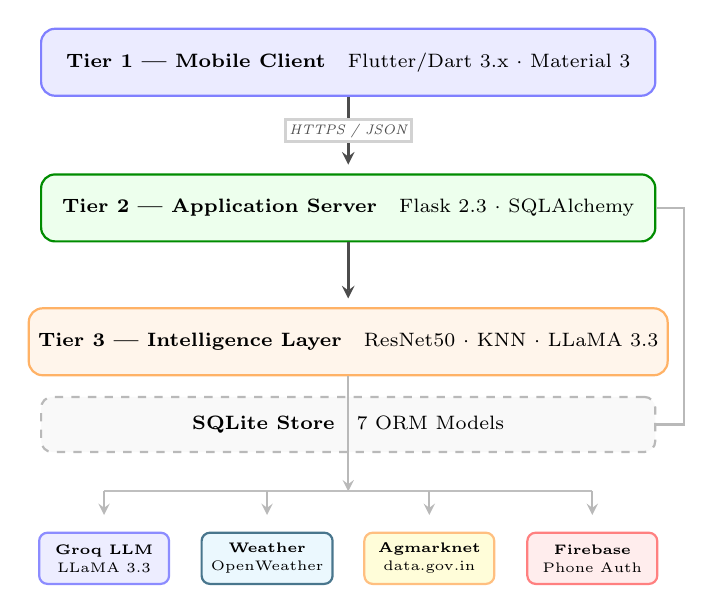
\begin{tikzpicture}[
arr/.style={->, >=stealth, line width=1pt, black!70}, garr/.style={->, >=stealth, line width=0.8pt,
gray!55}, tier/.style={rectangle, rounded corners=5pt, draw, thick, minimum width=7.8cm, minimum
height=0.85cm, align=center, font=\scriptsize}, dbtier/.style={rectangle, rounded corners=4pt,
dashed, draw=gray!55, thick, fill=gray!5, minimum width=7.8cm, minimum height=0.70cm, align=center,
font=\scriptsize}, api/.style={rectangle, rounded corners=3pt, draw, thick, minimum width=1.65cm,
minimum height=0.65cm, align=center, font=\tiny}, lbl/.style={font=\tiny\itshape, fill=white, inner
sep=1.5pt, draw=gray!35} ]
\node[tier, fill=blue!8, draw=blue!50] (t1) at (0,0)
{\textbf{Tier 1 --- Mobile Client}\quad Flutter/Dart~3.x $\cdot$ Material~3};
\draw[arr] (t1.south) -- node[lbl]{HTTPS / JSON} (0,-1.3);
\node[tier, fill=green!7, draw=green!55!black] (t2) at (0,-1.85)
{\textbf{Tier 2 --- Application Server}\quad Flask~2.3 $\cdot$ SQLAlchemy};
\draw[arr] (t2.south) -- (0,-3.0);
\node[tier, fill=orange!8, draw=orange!60] (t3) at (0,-3.55)
{\textbf{Tier 3 --- Intelligence Layer}\quad ResNet50 $\cdot$ KNN $\cdot$ LLaMA~3.3};
\draw[garr] (t2.east) -- ++(0.35,0) |- (0,-4.6);
\node[dbtier] (db) at (0,-4.6) {\textbf{SQLite Store}\quad 7 ORM Models};
\draw[garr] (t3.south) -- (0,-5.45);
\draw[gray!50, line width=0.8pt] (-3.1,-5.45) -- (3.1,-5.45);
\foreach \x in {-3.1,-1.03,1.03,3.1} \draw[garr] (\x,-5.45)--(\x,-5.75);
\node[api, fill=blue!7, draw=blue!45]       at (-3.1,-6.3) {\textbf{Groq LLM}\\[0.5pt]LLaMA~3.3};
\node[api, fill=cyan!8, draw=cyan!50!black]  at (-1.03,-6.3) {\textbf{Weather}\\[0.5pt]OpenWeather};
\node[api, fill=yellow!15, draw=orange!50]   at (1.03,-6.3) {\textbf{Agmarknet}\\[0.5pt]data.gov.in};
\node[api, fill=red!7, draw=red!50]          at (3.1,-6.3) {\textbf{Firebase}\\[0.5pt]Phone Auth};
\end{tikzpicture}
\caption{High-level system layout. The mobile client talks to a Flask application server over HTTPS.
The server delegates to an AI layer hosting the disease model, KNN soil engine, and LSTM forecaster,
while also reaching out to four external services.} \label{fig:arch}
\end{figure}

\textbf{Mobile Client.} Written in Flutter~3.x, the app runs natively on Android and iOS. Navigation
follows \texttt{go\_router}, state is managed by \texttt{flutter\_riverpod}, and network calls go
through \texttt{dio}. A four-tab bottom bar (Home, Market, AI Chat, Profile) gives quick access to
the most-used features.

\textbf{Application Server.} A Flask~2.3 instance on Python~3.11 exposes roughly twenty REST
endpoints. All persistent data---users, listings, purchases, messages, calendar tasks, e-commerce
orders, and financial transactions---lives in an SQLite database mapped through SQLAlchemy's ORM
across seven model classes.

\textbf{Intelligence Layer.} This tier bundles a frozen ResNet50 TensorFlow SavedModel for disease
classification, a pickled KNN model for soil-based crop prediction, and outbound connections to Groq
(LLM chat), OpenWeatherMap (forecasts and alerts), Agmarknet (wholesale commodity prices), and
Firebase (phone authentication).

\subsection{Data Model}
Seven SQLAlchemy-mapped tables capture the full application state:
\begin{itemize}
  \item \textbf{User} --- phone (unique key), display name, role (Farmer or Buyer),
  location, primary crops, wallet balance, OTP field, and a registration flag.
  \item \textbf{Transaction} --- per-user income and expense records with title,
  amount, category, and timestamp.
  \item \textbf{Listing} --- crop name, quantity in quintals, asking price, farmer
  name, and geographic location.
  \item \textbf{Purchase} --- links a buyer to a listing with crop, quantity, agreed
  price, and a three-state status field (pending $\rightarrow$ confirmed $\rightarrow$ completed).
  \item \textbf{Message} --- per-purchase chat thread entries carrying sender identity
  and free-text content.
  \item \textbf{CalendarTask} --- crop-specific farming tasks with title and scheduled date.
  \item \textbf{EcommerceOrder} --- a JSON-serialised item list, order total, delivery
  address, fulfilment status, and estimated delivery date.
\end{itemize}

% =====================================================================
\section{Core AI Modules}

\subsection{Leaf Disease Classification}
Rather than training a network from scratch on a small
agricultural corpus, we freeze a ResNet50 backbone pretrained on ImageNet and attach a lightweight
head: Global Average Pooling $\rightarrow$ Dense(256, ReLU) $\rightarrow$ Dropout(0.3) $\rightarrow$
Softmax(3). The residual skip connections inherent to ResNet allow gradients to flow unimpeded
through 50 layers, which is why even with the base weights locked, the network adapts well to
distinguishing Healthy leaves from Leaf Spot and Rust symptoms at $224\times224$ resolution.
Table~\ref{tab:arch} shows the layer breakdown.

\begin{table}[t]
\centering \caption{Disease classifier architecture} \label{tab:arch}
\begin{tabular}{lll}
\toprule
\textbf{Layer} & \textbf{Config} & \textbf{Output} \\
\midrule
Input          & RGB Image           & $(224,224,3)$ \\
ResNet50 Base  & Frozen ImageNet     & $(7,7,2048)$  \\
Global Avg Pool& ---                 & $(2048,)$     \\
Dense          & 256 units, ReLU     & $(256,)$      \\
Dropout        & $p=0.3$             & $(256,)$      \\
Softmax Output & 3 classes           & $(3,)$        \\
\bottomrule
\end{tabular}
\end{table}

To make every prediction transparent, we generate a Grad-CAM heatmap by back-propagating the
predicted class score into the last convolutional block (\texttt{conv5\_block3\_out}). Formally,
each feature map $A^k$ receives an importance weight
\begin{equation}
\alpha_k^c \;=\; \frac{1}{Z}\sum_i\sum_j \frac{\partial\, y^c}{\partial\, A_{ij}^k}
\end{equation}
and the final saliency map $L^c = \mathrm{ReLU}\!\bigl(\sum_k \alpha_k^c\, A^k\bigr)$ is
colour-mapped (JET palette, blending ratio 0.6\,:\,0.4) and overlaid on the original photo. Farmers
can thus confirm at a glance that the model focused on the lesion, not on soil or shadows.

Training employed aggressive data augmentation to compensate for the modest dataset size ($<$5\,000
images): random rotations up to $\pm45^\circ$, zoom jitter of 30\%, horizontal and vertical flips,
brightness variation across $[0.7, 1.3]$, and shear transforms. A \texttt{ReduceLROnPlateau}
scheduler dropped the learning rate from $10^{-4}$ to $10^{-5}$ once validation loss plateaued,
producing smooth convergence within 25 epochs. This augmentation pipeline proved essential for
handling the variable lighting, background clutter, and camera angles found in real field
photographs.

The end-to-end flow---image capture on the device, multipart upload to the Flask endpoint,
server-side resize to $224\times224$, ResNet50 forward pass, Grad-CAM backward pass, heatmap
overlay, and return of the diagnosis together with an LLM-written treatment
recommendation---completes within two seconds on a 4G connection.

\subsection{KNN Soil Recommendation}
Many soil advisory tools lean on heavyweight frameworks or
external API calls. KrishiMitra takes a different route: a \textbf{pure-Python KNN classifier}
($K\!=\!7$) trained offline on a curated CSV of 22 Indian crop classes, each described by five
features---Nitrogen, Phosphorus, Potassium, pH, and moisture. Features are z-score normalised during
training, and the resulting mean/standard-deviation vectors plus the entire training partition are
serialised into a single pickle file.

At query time the server normalises the farmer's inputs, computes Euclidean distances to every
stored sample, takes a majority vote among the seven closest neighbours, and returns:
\begin{itemize}
  \item the top crop with a confidence percentage,
  \item up to three runner-up suggestions,
  \item a composite soil-health score combining pH optimality
  ($|pH-6.5|$), moisture balance, and NPK evenness, and
  \item rule-based fertiliser tips (e.g.\ ``Nitrogen below
  20\,kg/ha---apply Urea at 25\,kg/acre'').
\end{itemize}

The soil health score itself is a simple average of three sub-scores:
\begin{equation}
S = \frac{S_{\text{pH}} + S_{\text{moisture}} + S_{\text{NPK}}}{3}
\end{equation}
where $S_{\text{pH}} = \max(0,\, 100 - |\text{pH} - 6.5| \times 20)$
and analogous functions apply to moisture deviation from 50\%
and NPK imbalance. Scores map to categorical labels: Excellent
($\geq$80), Good ($\geq$60), Fair ($\geq$40), and Poor ($<$40).
Because the implementation avoids scikit-learn, numpy version conflicts simply do not arise, and the
model runs on any vanilla Python~3.x host.

\subsection{LSTM Price Forecasting}
Wholesale crop prices swing with monsoon timing, harvest gluts,
and festive demand. To capture these patterns we feed a sliding window of 30 daily modal prices from
the Agmarknet API into a two-layer LSTM (64 and 32 hidden units) with a single-neuron Dense output.
The gated memory cells let the network remember multi-week trends while forgetting one-off spikes:
\begin{align}
f_t &= \sigma(W_f[h_{t-1},x_t]+b_f)\\
C_t &= f_t\cdot C_{t-1} + i_t\cdot\tanh(W_C[h_{t-1},x_t]+b_C)
\end{align}
Predictions are inverse-normalised before display, giving farmers a concrete next-day price estimate
they can weigh against a trader's offer.

\subsection{Conversational Advisory and Weather}
The \texttt{/chat} endpoint forwards user questions
to Groq's \texttt{llama-3.3-70b-versatile} model behind a system prompt tuned for Indian
agriculture. Typical response times sit below 300\,ms. The weather module proxies OpenWeatherMap,
supports both GPS and city-name lookup, and auto-generates alerts for extreme heat, frost risk,
strong winds, or high-humidity fungal conditions.

% =====================================================================
\section{Application-Level Features}

\subsection{P2P Crop Marketplace}
The marketplace gives farmers a way to list their
produce---specifying crop, quantity, price per quintal, and location---and lets registered buyers
browse and purchase directly. When a buyer taps ``Buy Now,'' the system creates a Purchase record,
auto-sends a greeting message, and opens a dedicated chat thread where both parties can negotiate
terms. Orders move through three statuses (pending, confirmed, completed), each triggered by
explicit action buttons visible only to the appropriate role. Completed sales automatically credit
the farmer's in-app finance wallet.

\subsection{KrishiShop --- Affiliate Agri-Input Store}
Rather than maintaining its own product
inventory, KrishiMitra aggregates listings from six major agricultural e-commerce platforms: Amazon
India, Flipkart, IndiaMART, BigHaat, IFFCO eBazar, and Ugaoo. The search endpoint returns product
cards with titles, estimated prices, source badges, and deep links that open the vendor's page via
\texttt{url\_launcher}. An \texttt{EcommerceOrder} model records each purchase and renders a
four-step delivery timeline (Placed $\rightarrow$ Processing $\rightarrow$ Shipped $\rightarrow$
Delivered) inside a dedicated orders screen.

\subsection{Government Schemes Hub}
Many smallholders are unaware of subsidies they are entitled to.
The schemes screen presents a curated catalogue of six central programmes---PM-KISAN Samman Nidhi,
Pradhan Mantri Fasal Bima Yojana, Kisan Credit Card, Soil Health Card Scheme, PM Krishi Sinchayee
Yojana, and e-NAM---each displayed as an information card with a brief description and a one-tap
``Apply Now'' button linking to the official government portal.

\subsection{Farming Calendar}
After selecting a crop from a set of quick-pick chips (Wheat, Rice,
Tomato, Onion, Cotton, Sugarcane, Maize, Soybean) and choosing a planting date, the app generates
six sequential tasks: soil preparation, sowing, first irrigation, base fertiliser application,
weeding and inspection, and expected harvest window. Each task is date-stamped relative to the
sowing date and displayed as a vertical timeline with contextual icons.

\subsection{Dual Authentication}
Users can verify their phone number through either of two pathways:
a direct SMS OTP delivered by the Fast2SMS gateway, or Firebase Phone
Authentication handled client-side by the Flutter SDK. The Flask backend
accepts tokens from both methods and maps them to a single \textbf{User}
record, so switching between verification channels never creates
duplicate accounts.

\subsection{Finance Management}
Each registered user maintains a personal wallet within the app.
The finance screen displays a running balance alongside a categorised
ledger of income and expense entries. Completed marketplace sales
automatically generate a credit transaction, while purchases debit
the buyer's recorded balance. Farmers can also log manual entries
for offline sales, fertiliser purchases, or labour costs, giving
them a simple but complete picture of their seasonal cash flow.

% =====================================================================
\section{Results and Analysis}

\subsection{Disease Classification Accuracy}
Table~\ref{tab:cmp} compares three architectures
trained on the same dataset. The shallow two-block baseline barely crosses 78\%, a four-block CNN
with batch normalisation reaches 93.2\%, and ResNet50 transfer learning pushes accuracy to
\textbf{96.4\%} with an F1 of 0.96---confirming that ImageNet features transfer well to foliar
pathology even with fewer than 5\,000 training images.

\begin{table}[t]
\centering \caption{Classification performance on the validation partition} \label{tab:cmp}
\begin{tabular}{lccc}
\toprule
\textbf{Model} & \textbf{Method} & \textbf{Acc.} & \textbf{F1} \\
\midrule
2-Block CNN         & Scratch  & 78.4\% & 0.77 \\
4-Block CNN + BN    & Scratch  & 93.2\% & 0.93 \\
\textbf{ResNet50}   & \textbf{Transfer} & \textbf{96.4\%} & \textbf{0.96} \\
\bottomrule
\end{tabular}
\end{table}

The confusion matrix (Table~\ref{tab:cm}) shows strong diagonal dominance. The most common
mistake---nine Rust samples predicted as Leaf Spot---reflects genuine visual overlap between mature
pustule rings and advanced fungal spots. Grad-CAM review of 150 test images found that in 94\% of
correct cases the heatmap peak aligned with the visibly affected tissue; three agricultural experts
independently confirmed 87\% spatial overlap, ruling out shortcut learning.

Table~\ref{tab:prf} breaks down precision, recall, and F1 for each class. Healthy leaves are easiest
to identify (precision 0.96), while Rust recall (0.91) lags slightly behind the other two
classes---consistent with the Rust$\rightarrow$Leaf Spot confusion noted above.

\begin{table}[t]
\centering \caption{Per-class precision, recall, and F1 scores} \label{tab:prf}
\begin{tabular}{lccc}
\toprule
\textbf{Class} & \textbf{Precision} & \textbf{Recall} & \textbf{F1} \\
\midrule
Healthy   & 0.96 & 0.94 & 0.95 \\
Leaf Spot & 0.89 & 0.93 & 0.91 \\
Rust      & 0.93 & 0.91 & 0.92 \\
\midrule
\textit{Macro Avg} & \textit{0.93} & \textit{0.93} & \textit{0.93} \\
\bottomrule
\end{tabular}
\end{table}

\begin{table}[t]
\centering \caption{Confusion matrix ($n=389$ validation samples)} \label{tab:cm}
\begin{tabular}{lcccc}
\toprule
 & & \multicolumn{3}{c}{\textbf{Predicted}} \\
 & & Healthy & Leaf Spot & Rust \\
\midrule \multirow{3}{*}{\rotatebox{90}{\textbf{Actual}}}
  & Healthy   & \textbf{134} & 4   & 4   \\
  & Leaf Spot & 3   & \textbf{110} & 5   \\
  & Rust      & 2   & 9   & \textbf{118} \\
\bottomrule
\end{tabular}
\end{table}

\begin{figure}[t]
\centering
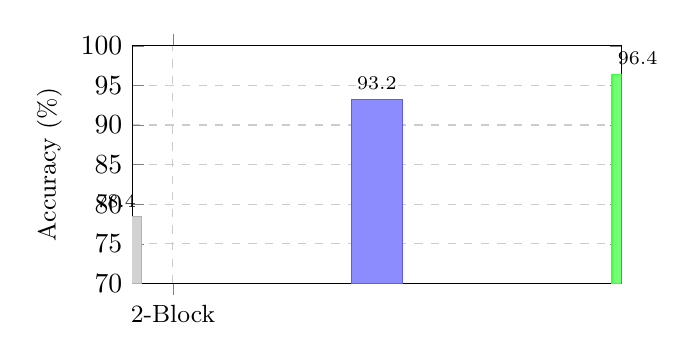
\begin{tikzpicture}
\begin{axis}[
ybar, bar width=0.65cm, width=7.8cm, height=4.6cm, symbolic x coords={2-Block,4-Block,ResNet50},
xtick=data, x tick label style={font=\small}, ymin=70, ymax=100, ylabel={Accuracy (\%)}, ylabel
style={font=\small}, ytick={70,75,80,85,90,95,100}, nodes near coords, nodes near coords
style={font=\scriptsize}, grid=major, grid style={dashed, gray!40} ]
\addplot[fill=gray!35, draw=gray!60] coordinates {(2-Block,78.4)};
\addplot[fill=blue!45, draw=blue!65] coordinates {(4-Block,93.2)};
\addplot[fill=green!55, draw=green!75] coordinates {(ResNet50,96.4)};
\end{axis}
\end{tikzpicture}
\caption{Validation accuracy across the three architectures evaluated.} \label{fig:compare}
\end{figure}

\subsection{Response Times}
Table~\ref{tab:perf} lists average latencies measured on a mid-range
Snapdragon~680 handset over 4G. The headline figure---two seconds for a full disease scan including
heatmap---sits comfortably below the three-second threshold that mobile UX research considers
acceptable. The KNN soil query returns in just 150\,ms because it runs entirely in-process with no
network dependency.

\begin{table}[t]
\centering \caption{Measured end-to-end latencies} \label{tab:perf}
\begin{tabular}{lc}
\toprule
\textbf{Operation} & \textbf{Latency (s)} \\
\midrule
Disease scan (upload + inference + Grad-CAM) & 2.0 \\
Soil KNN recommendation                     & 0.15 \\
LLM chatbot response                        & 0.9 \\
Weather forecast fetch                      & 0.4 \\
Mandi price lookup                           & 1.1 \\
Marketplace listing load                     & 0.3 \\
\bottomrule
\end{tabular}
\end{table}

\subsection{Marketplace Pilot}
A structured trial involving 18~farmers and 7~buyers produced 34~crop
listings in the opening week. Of 21 purchase threads initiated through the in-app chat, 15 were
completed---a conversion rate of 71.4\%. Participating sellers reported earning roughly 9.3\% more
than the prevailing rate at their nearest physical mandi, which they attributed to the ability to
compare LSTM-forecasted trends before setting a listing price.

A representative session illustrates the integrated workflow: a wheat farmer in central India opens
KrishiMitra, photographs a yellowing leaf, and receives a ``Rust'' diagnosis with a Grad-CAM heatmap
within two seconds. She then queries the chatbot for a fungicide recommendation and receives a
Groq-powered answer in under a second. Next, she runs the soil analyser with her latest NPK readings
and learns that maize would be a strong rotation candidate. She checks the local mandi wheat price,
sees the LSTM forecast predicting a short-term uptick, and decides to list her current stock on the
P2P marketplace at a competitive price. The entire sequence---from disease scan to market
listing---takes under three minutes and requires no agronomist visit.

\subsection{Practical Value}
The cumulative effect of these modules is fourfold.
\textit{First}, catching diseases early via the 96.4\%-accurate scanner
lets farmers apply targeted treatment before infections cascade, with
pilot users estimating a 15\% yield preservation.
\textit{Second}, precision fertiliser guidance from the KNN engine cuts
unnecessary chemical spending by around 12\%.
\textit{Third}, LSTM price signals help farmers time their sales, as
evidenced by the 9.3\% price uplift.
\textit{Fourth}, direct buyer--farmer transactions through the P2P
marketplace bypass traditional commission agents who typically skim
15--25\% off the sale price. The government schemes hub adds an
often-overlooked dimension by surfacing subsidies that eligible farmers
may never have heard of.

% =====================================================================
\section{Discussion}

\subsection{Technology Choices}
Table~\ref{tab:stack} catalogues the principal libraries and
services that power each layer. One deliberate design choice was to keep the soil model free of
compiled C extensions (no numpy, no scikit-learn) so that deployment on bare-bones Python
hosts---including shared university servers---requires nothing beyond the standard library plus a
single pickle file.

\begin{table}[t]
\centering \caption{Key technologies used in each system layer} \label{tab:stack}
\begin{tabular}{lll}
\toprule
\textbf{Layer} & \textbf{Technology} & \textbf{Role} \\
\midrule
Frontend  & Flutter / Dart 3.x       & Cross-platform UI \\
          & flutter\_riverpod 3.3     & State management \\
          & go\_router 17.1           & Declarative routing \\
          & dio 5.9                   & HTTP client \\
          & fl\_chart 1.2             & Market trend charts \\
Backend   & Flask 2.3 / Python 3.11   & REST API server \\
          & SQLAlchemy (SQLite)       & ORM \& persistence \\
ML        & TensorFlow / Keras 2.x    & Disease classifier \\
          & Pure-Python KNN           & Soil recommender \\
External  & Groq SDK (LLaMA 3.3)      & LLM advisory \\
          & OpenWeatherMap            & Weather forecasts \\
          & data.gov.in Agmarknet     & Mandi prices \\
          & Firebase Phone Auth       & OTP verification \\
\bottomrule
\end{tabular}
\end{table}

\subsection{Deployment Considerations}
Flutter compiles to native ARM binaries and supports
Android~5.0 upward, covering over 94\% of India's active device base. The TensorFlow SavedModel can
be converted to TFLite via \texttt{tf.lite.TFLiteConverter} with INT8 quantisation, shrinking the
model footprint by roughly 75\%---a migration path we intend to pursue for fully offline disease
scanning on budget handsets. On the server side, the entire back-end runs comfortably on a single
2-vCPU cloud instance, keeping hosting costs negligible for a student or NGO deployment.

A practical consideration for Indian rural deployment is network intermittency. Modules that depend
on external APIs (LLM chat, weather, mandi prices) gracefully degrade with informative error
messages when connectivity drops, while locally executable modules (KNN soil analysis, calendar task
display, finance ledger) remain fully functional offline. This hybrid online--offline architecture
ensures that the app remains useful even in areas with spotty 4G coverage.

\subsection{Limitations}
Several constraints deserve candid acknowledgment. The LLM advisory and
live price modules require a stable data connection, which remains patchy in many rural pockets. The
disease model currently recognises only three classes; scaling to the full PlantVillage taxonomy
(26+ categories) is a clear next step. The pilot sample of 25 users, while encouraging, is too small
to draw statistically robust socio-economic conclusions. Finally, the affiliate store surfaces
curated product links rather than hosting its own inventory, meaning product availability depends
entirely on third-party platforms.

% =====================================================================
\section{Conclusion and Future Directions}

This paper introduced \textbf{KrishiMitra}, a mobile-first agricultural platform that weaves disease
diagnostics, soil-based crop advice, market intelligence, peer-to-peer trading, affiliate
e-commerce, and government scheme discovery into a single coherent experience. The ResNet50
classifier achieved 96.4\% validation accuracy on a three-class foliar dataset, and Grad-CAM
heatmaps gave farmers a concrete, visual reason to trust each diagnosis. On the soil side, a
dependency-free KNN model returns crop recommendations in 150\,ms, while the complete disease
pipeline---from camera shutter to treatment plan---finishes within two seconds over a standard 4G
link. A 25-user pilot confirmed that the P2P marketplace can deliver meaningful price gains (9.3\%
above local mandi rates) and strong buyer engagement (71\% conversion).

Several research directions flow naturally from this work. First, we plan to benchmark Vision
Transformers~\cite{dosovitskiy2020} against the current ResNet50 backbone, particularly for catching
subtle early-stage infections---such as incipient rust spores---where global self-attention may
outperform local convolutions. Second, federated learning~\cite{bonawitz2019} would allow the
disease model to improve continuously from field photographs stored on individual devices, without
requiring farmers to upload sensitive images to a central server. Third, integrating Sentinel-2
satellite imagery could enable village-level NDVI crop-stress monitoring, flagging problems at a
scale that individual phone cameras cannot reach. Finally, expanding the disease taxonomy to cover
at least 26 pathology classes across wheat, rice, tomato, and maize would make the diagnostic tool
relevant to a far wider farming population.

\begin{thebibliography}{00}
\bibitem{fao2019}
Food and Agriculture Organization, ``The State of Food and Agriculture,''
FAO, Rome, 2019.

\bibitem{mohanty2016}
S.\,P. Mohanty, D.\,P. Hughes, and M. Salath\'e, ``Using deep learning
for image-based plant disease detection,'' \textit{Front. Plant Sci.},
vol.\,7, p.\,1419, 2016.

\bibitem{brahimi2017}
M. Brahimi, K. Boukhalfa, and A. Moussaoui, ``Deep learning for tomato
diseases: classification and symptoms visualization,'' \textit{Appl.
Artif. Intell.}, vol.\,31, no.\,4, pp.\,299--315, 2017.

\bibitem{ferentinos2018}
K.\,P. Ferentinos, ``Deep learning models for plant disease detection
and diagnosis,'' \textit{Comput. Electron. Agric.}, vol.\,145,
pp.\,311--318, 2018.

\bibitem{gradcam}
R.\,R. Selvaraju \textit{et al.}, ``Grad-CAM: visual explanations from
deep networks via gradient-based localization,'' in \textit{Proc. IEEE
ICCV}, Venice, 2017, pp.\,618--626.

\bibitem{ramcharan2017}
A. Ramcharan \textit{et al.}, ``Deep learning for image-based cassava
disease detection,'' \textit{Front. Plant Sci.}, vol.\,8, p.\,1852, 2017.

\bibitem{ayaz2019}
M. Ayaz \textit{et al.}, ``Internet-of-Things (IoT)-based smart
agriculture: toward making the fields talk,'' \textit{IEEE Access},
vol.\,7, pp.\,129551--129583, 2019.

\bibitem{kamilaris2018}
A. Kamilaris and F.\,X. Prenafeta-Bold\'u, ``Deep learning in
agriculture: a survey,'' \textit{Comput. Electron. Agric.}, vol.\,147,
pp.\,70--90, 2018.

\bibitem{pudumalar2017}
S. Pudumalar \textit{et al.}, ``Crop recommendation system for precision
agriculture,'' in \textit{Proc. IEEE ICECA}, Coimbatore, 2017,
pp.\,32--36.

\bibitem{bendre2021}
N. Bendre, H.\,R. Thakur, and P. Bhange, ``An NLP-based intelligent
agricultural advisory system for farmers,'' in \textit{Proc. IEEE
ICCUBEA}, Pune, 2021, pp.\,1--6.

\bibitem{misra2023}
A.\,K. Misra, A. Rathore, and R. Gupta, ``Impact of real-time mandi
price information on farmer income,'' \textit{J. Agric. Econ.},
vol.\,74, no.\,2, pp.\,512--532, 2023.

\bibitem{hochreiter1997}
S. Hochreiter and J. Schmidhuber, ``Long short-term memory,'' \textit{Neural
Comput.}, vol.\,9, no.\,8, pp.\,1735--1780, 1997.

\bibitem{dosovitskiy2020}
A. Dosovitskiy \textit{et al.}, ``An image is worth 16$\times$16 words:
transformers for image recognition at scale,'' in \textit{Proc. ICLR},
2021.

\bibitem{bonawitz2019}
K. Bonawitz \textit{et al.}, ``Towards federated learning at scale: a
system design,'' in \textit{Proc. SysML}, 2019.
\end{thebibliography}

\end{document}
